\documentclass[11pt]{article}

\usepackage[margin=1in]{geometry}
\usepackage[T1]{fontenc}
\usepackage[utf8]{inputenc}
\usepackage{lmodern}
\usepackage{microtype}
\usepackage[table]{xcolor}
\usepackage{amsmath,amssymb,mathtools,bm}
\usepackage{booktabs,array,longtable,tabularx}
\usepackage{hyperref}
\usepackage{enumitem}
\usepackage{fancyhdr}
\usepackage{titlesec}
\usepackage{tcolorbox}
\usepackage{ragged2e}
\usepackage{setspace}
\hypersetup{colorlinks=true,linkcolor=blue!45!black,urlcolor=blue!45!black,citecolor=blue!45!black}
\definecolor{TitleBlue}{HTML}{163A5F}
\definecolor{AccentTeal}{HTML}{2D6F73}
\definecolor{SoftBlue}{HTML}{EAF3F8}
\definecolor{SoftTeal}{HTML}{EDF8F6}
\definecolor{SoftGray}{HTML}{F5F7FA}
\pagestyle{fancy}
\fancyhf{}
\lhead{PINN\_M3DC1}
\rhead{Project Plan}
\cfoot{\thepage}
\fancypagestyle{plain}{%
  \fancyhf{}%
  \lhead{PINN\_M3DC1}%
  \rhead{Project Plan}%
  \cfoot{\thepage}%
}
\setlength{\headheight}{14pt}
\setlength{\parskip}{0.45em}
\setlength{\parindent}{0pt}
\onehalfspacing
\numberwithin{equation}{section}
\titleformat{\section}{\Large\bfseries\color{TitleBlue}}{\thesection}{0.6em}{}
\titleformat{\subsection}{\large\bfseries\color{AccentTeal}}{\thesubsection}{0.6em}{}
\newtcolorbox{overviewbox}{colback=SoftBlue,colframe=TitleBlue,boxrule=0.8pt,arc=2mm,left=3mm,right=3mm,top=2mm,bottom=2mm}
\newtcolorbox{notebox}{colback=SoftGray,colframe=AccentTeal,boxrule=0.6pt,arc=2mm,left=3mm,right=3mm,top=2mm,bottom=2mm}
\newcommand{\DocTitle}[3]{%
\begin{center}
{\LARGE \bfseries \color{TitleBlue} #1}\\[0.5em]
{\large \color{AccentTeal} #2}\\[0.8em]
{\normalsize #3}
\end{center}
\vspace{0.5em}}
\newcommand{\ProjectTOC}{\vspace{0.5em}{\hypersetup{linkcolor=TitleBlue}\tableofcontents}\vspace{0.8em}}
\allowdisplaybreaks

\usepackage{tikz}
\usetikzlibrary{arrows.meta,positioning,calc,shapes.geometric,fit}
\usepackage{caption}
\usepackage{multirow}
\usepackage{makecell}
\usepackage{upquote}

\definecolor{WarningRed}{HTML}{9B2C2C}
\definecolor{WarmGold}{HTML}{B7791F}
\definecolor{PaleGold}{HTML}{FFF8E6}
\definecolor{PaleRed}{HTML}{FFF1F1}
\definecolor{DeepGreen}{HTML}{276749}
\definecolor{Purple}{HTML}{5B3F8C}
\definecolor{PalePurple}{HTML}{F3EFFA}

\newtcolorbox{definitionbox}[1][]{
  colback=SoftTeal,colframe=AccentTeal,title={Definition#1},
  fonttitle=\bfseries,boxrule=0.7pt,arc=2mm,
  left=3mm,right=3mm,top=2mm,bottom=2mm}
\newtcolorbox{warningbox}[1][]{
  colback=PaleRed,colframe=WarningRed,title={Important distinction#1},
  fonttitle=\bfseries,boxrule=0.7pt,arc=2mm,
  left=3mm,right=3mm,top=2mm,bottom=2mm}
\newtcolorbox{checkpointbox}[1][]{
  colback=PaleGold,colframe=WarmGold,title={Validation checkpoint#1},
  fonttitle=\bfseries,boxrule=0.7pt,arc=2mm,
  left=3mm,right=3mm,top=2mm,bottom=2mm}
\newtcolorbox{conventionbox}[1][]{
  colback=SoftBlue,colframe=TitleBlue,title={Frozen Module 3 convention#1},
  fonttitle=\bfseries,boxrule=0.9pt,arc=2mm,
  left=3mm,right=3mm,top=2mm,bottom=2mm}
\newtcolorbox{resultbox}[1][]{
  colback=SoftTeal,colframe=DeepGreen,title={Required result#1},
  fonttitle=\bfseries,boxrule=0.8pt,arc=2mm,
  left=3mm,right=3mm,top=2mm,bottom=2mm}
\newtcolorbox{adapterbox}[1][]{
  colback=PalePurple,colframe=Purple,title={M3D-C1 adapter boundary#1},
  fonttitle=\bfseries,boxrule=0.8pt,arc=2mm,
  left=3mm,right=3mm,top=2mm,bottom=2mm}

\newcommand{\vect}[1]{\bm{#1}}
\newcommand{\mat}[1]{\bm{#1}}
\newcommand{\pd}{\partial}
\newcommand{\Lap}{\nabla_{\!\perp}^{2}}
\newcommand{\Laph}{\nabla_{\!\perp,h}^{2}}
\newcommand{\average}[1]{\left\langle #1\right\rangle}
\newcommand{\norm}[1]{\left\lVert #1\right\rVert}
\newcommand{\dataset}[1]{\texttt{/#1}}
\newcommand{\code}[1]{\texttt{#1}}

\pagestyle{fancy}
\fancyhf{}
\lhead{PINN\_M3DC1}
\rhead{Module 3 Physics Notes}
\cfoot{\thepage}
\fancypagestyle{plain}{%
  \fancyhf{}%
  \lhead{PINN\_M3DC1}%
  \rhead{Module 3 Physics Notes}%
  \cfoot{\thepage}%
}

\begin{document}
\hypersetup{pageanchor=false}

\begin{titlepage}
\centering
\vspace*{1.15cm}
{\Large\color{AccentTeal} PINN\_M3DC1}\par
\vspace{0.7cm}
{\Huge\bfseries\color{TitleBlue} Module 3}\par
\vspace{0.25cm}
{\LARGE\bfseries\color{TitleBlue} Full-Field Dataset Contracts and\\M3D-C1-Shaped Input/Output}\par
\vspace{0.9cm}
{\large A textbook-style scientific data specification for auditable reduced-MHD surrogate learning}\par
\vfill
\begin{tcolorbox}[width=0.90\textwidth,colback=SoftBlue,colframe=TitleBlue,arc=2mm]
\centering
\textbf{Module purpose}\par
\vspace{0.35em}
Store accepted numerical fields, parameters, coordinates, provenance, and whole-case splits in explicit versioned schemas, then construct lossless full-field operator views for Modules 4 and 5 without changing the physical meaning fixed by Modules 1 and 2.
\end{tcolorbox}
\vfill
{\normalsize Version 1.1 \quad | \quad 11 August 2026}\par
\vspace{0.25cm}
{\small Physics and full-field data-contract note for the synthetic reduced-MHD proof of concept}\par
\end{titlepage}

\hypersetup{pageanchor=true}
\pagenumbering{roman}

\section*{Preface: why a data contract is part of the physics}

Module~2 produces verified numerical trajectories and freezes the revised downstream map
\begin{equation*}
\left(\psi_0(x,y),U_0(x,y),\eta,\nu,t\right)
\longmapsto
\left(\psi(x,y,t),U(x,y,t)\right).
\end{equation*}
Module~3 determines whether those trajectories remain scientifically intelligible after they are written to disk, combined into a dataset, split for learning, transformed for optimization, packed into full-field tensors, read by another programming language, and eventually compared with genuine M3D-C1 exports. The learning object is therefore no longer one coordinate row. It is a complete two-dimensional numerical-field input paired with a complete two-dimensional numerical-field target at a declared time.

A file format alone cannot answer these questions. An array of numbers does not identify which axis is time, whether current means $J=-\Lap\psi$ or $J=+\Lap\psi$, whether the rightmost spatial endpoint is duplicated, whether a field is dimensional or nondimensional, whether a case passed convergence checks, or whether preprocessing used the test set. Those facts determine the scientific meaning of every number. The \textbf{data contract} is the set of rules that makes that meaning explicit and machine-checkable.

The initials \textbf{I/O} mean \emph{input/output}: how information enters and leaves a computational component. \textbf{HDF5} means Hierarchical Data Format version~5, a format that organizes multidimensional datasets, groups, and attributes. \textbf{Schema} means a versioned specification of required names, types, shapes, meanings, and relationships. \textbf{Provenance} means the recorded history of how an artifact was produced. A \textbf{full-field operator example} contains complete numerical arrays rather than isolated scalar samples. \textbf{Normalization} here can mean either physical nondimensionalization or a later numerical transform for neural-network training; these are different operations and must remain distinguishable.

\begin{warningbox}
``M3D-C1-shaped'' describes the architecture of the workflow: coordinates or mesh information, parameters, time-dependent numerical fields, metadata, diagnostics, and an adapter boundary. The revised full-field tensors make this interface more field-oriented, but they do not make the synthetic Cartesian variables numerically equivalent to M3D-C1 variables, make the geometries agree, or validate an M3D-C1 surrogate.
\end{warningbox}

\subsection*{The main dependency chain}

\begin{center}
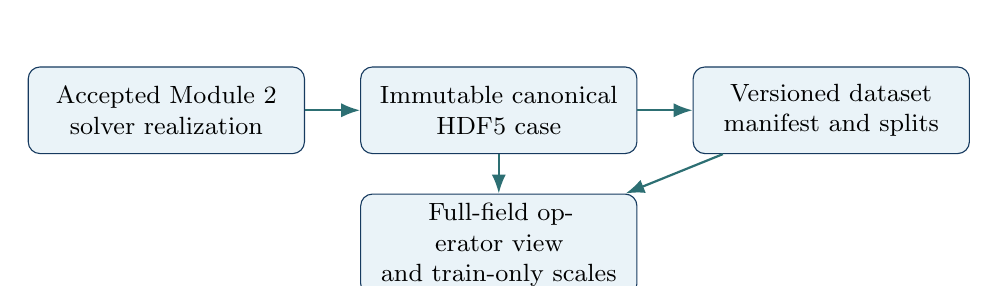
\begin{tikzpicture}[
  node distance=5mm and 7mm,
  box/.style={draw=TitleBlue,rounded corners=1.5mm,fill=SoftBlue,align=center,
              minimum height=11mm,text width=0.27\textwidth,font=\small},
  arrow/.style={-{Latex[length=2.4mm]},thick,draw=AccentTeal}]
\node[box] (solver) {Accepted Module 2\\solver realization};
\node[box, right=of solver] (case) {Immutable canonical\\HDF5 case};
\node[box, right=of case] (manifest) {Versioned dataset\\manifest and splits};
\node[box, below=of case] (processed) {Full-field operator view\\and train-only scales};
\draw[arrow] (solver) -- (case);
\draw[arrow] (case) -- (manifest);
\draw[arrow] (manifest) -- (processed);
\draw[arrow] (case) -- (processed);
\end{tikzpicture}
\end{center}

The reference case is never overwritten by a preprocessing step. A learning-ready representation is a derived artifact whose parent, transforms, split manifest, and checksums are recorded.

\subsection*{Learning objectives}

After working through this module, the reader should be able to:
\begin{enumerate}[label=\arabic*.]
  \item explain why array names, axes, and grid registration are physical statements rather than clerical details;
  \item distinguish a physical case, numerical realization, snapshot, grid point, and full-field operator example;
  \item state the exact canonical shapes and meanings of $\psi$, $U$, $J$, and $\omega$;
  \item explain why accepted reference fields remain unstandardized, unrendered, and immutable;
  \item design an HDF5 hierarchy that preserves coordinates, fields, parameters, diagnostics, verification, and provenance;
  \item assign stable physical-case, realization, initial-state, and operator-example identities;
  \item construct whole-trajectory training, validation, interpolation-test, and extrapolation-test partitions before extracting target times;
  \item identify leakage caused by time-snapshot splitting, duplicate realizations, or test-fitted preprocessing;
  \item construct $(\psi_0,U_0,\eta,\nu,t)\mapsto(\psi_t,U_t)$ from raw numerical arrays without rendering images;
  \item pack fields and scalar context into reversible tensor channels while preserving the parent HDF5 axes and values;
  \item explain why $A_0$ remains case metadata even though the complete $U_0$ field already encodes it;
  \item distinguish the number of physical trajectories from the much larger number of time-conditioned operator pairs;
  \item define common-grid and resolution rules appropriate to a full-field neural operator;
  \item fit and store invertible field and scalar transforms using training cases only;
  \item preserve the spatial-grid metadata needed for spectral physics residuals in Module~5;
  \item verify Python--MATLAB field-array and tensor-packing parity;
  \item describe the explicit translation work required for genuine M3D-C1 data; and
  \item state precisely which claims a Module~3 operator dataset can and cannot support.
\end{enumerate}

\ProjectTOC
\clearpage
\pagenumbering{arabic}

\section{Scientific role and acceptance boundary}
\label{sec:role}

\subsection{The object produced by Module 3}

For a physical parameter vector
\begin{equation}
\vect{\mu}_c=(\eta_c,\nu_c,A_{0,c}),
\end{equation}
Module~2 approximates one accepted reduced-MHD trajectory. Module~3 creates an auditable release
\begin{equation}
\mathcal D=\left(\mathcal C,\mathcal M,\mathcal S,\mathcal V,\mathcal T\right),
\label{eq:dataset_object}
\end{equation}
where
\begin{itemize}
  \item $\mathcal C$ is a set of accepted canonical case files;
  \item $\mathcal M$ is a manifest describing and indexing those files;
  \item $\mathcal S$ is an immutable whole-physical-case split assignment;
  \item $\mathcal V$ is a declared full-field operator view specifying how initial fields and target times become input-target tensors; and
  \item $\mathcal T$ is the set of declared, invertible preprocessing transforms fitted only from training cases.
\end{itemize}

For each accepted case and saved target time $t_n$, the primary version-1 operator example is
\begin{equation}
X_{c,n}=\left(\psi^{(c)}_0(\cdot,\cdot),U^{(c)}_0(\cdot,\cdot),\eta_c,\nu_c,t_n\right),
\qquad
Y_{c,n}=\left(\psi^{(c)}_n(\cdot,\cdot),U^{(c)}_n(\cdot,\cdot)\right).
\label{eq:operator_example}
\end{equation}
The dots mean the complete two-dimensional numerical arrays on the accepted grid. They do not mean images, contour plots, or isolated coordinate samples.

The manifest and operator-view specification are part of the scientific artifact. A directory of HDF5 files without an authoritative index does not define which files belong to a release, which are accepted, which target times form learning examples, or how they are partitioned.

\subsection{Four layers that must not be confused}

\begin{longtable}{p{0.19\textwidth}p{0.34\textwidth}p{0.37\textwidth}}
\toprule
Layer & Object & Main question \\
\midrule
\endfirsthead
\toprule
Layer & Object & Main question \\
\midrule
\endhead
Physical model & Continuous fields and equations & What do $\psi,U,J,\omega,\eta,\nu,A_0$ mean? \\
Numerical realization & Finite arrays from one solver run & Which grid, time step, integrator, precision, and verification status produced them? \\
Serialized reference & HDF5 datasets plus metadata & Can another reader reconstruct the same logical arrays and meanings? \\
Learning view & Whole-field input-target tensors derived from accepted trajectories & Which split, target-time rule, channel layout, grid class, scales, and inverse transforms define the neural task? \\
\bottomrule
\end{longtable}

A neural preprocessing choice must not be written back into the physical-model layer. Similarly, changing a field sign cannot be treated as a harmless file-format revision.

\subsection{Acceptance inherited from Module 2}

Module~3 ingests only cases for which the Module~2 acceptance record is complete and true. At minimum, the case must have passed:
\begin{itemize}
  \item operator and sign tests;
  \item analytic or manufactured-solution checks;
  \item temporal and spatial convergence checks;
  \item spectral and current-sheet resolution checks;
  \item energy, periodicity, gauge, and topology checks;
  \item finite-value and complete-horizon checks; and
  \item Python--MATLAB parity at the declared level when parity is required for that release.
\end{itemize}

\begin{checkpointbox}
The Module~3 validator must fail closed. Missing acceptance metadata means ``not eligible,'' not ``probably accepted.'' A rejected or incomplete case may be retained for debugging, but it cannot appear in an accepted release manifest.
\end{checkpointbox}

\subsection{What Module 3 does not establish}

Module~3 does not prove that the solver equations are physically adequate for a stellarator, that a neural network has learned them, or that an M3D-C1 export can be interpreted through the same variables. It establishes a trustworthy interface for the stated synthetic model and a place where a future adapter can make every required translation explicit.

\section{Frozen physical semantics}
\label{sec:semantics}

\subsection{Domain, coordinates, and endpoint convention}

The version-1 domain is
\begin{equation}
\Omega=[0,L_x)\times[0,L_y),
\qquad L_x=L_y=2\pi.
\end{equation}
The spatial grids are
\begin{align}
x_i&=i\Delta x, & \Delta x&=L_x/N_x, & i&=0,\ldots,N_x-1,\\
y_j&=j\Delta y, & \Delta y&=L_y/N_y, & j&=0,\ldots,N_y-1.
\end{align}
The right endpoints $L_x$ and $L_y$ are not duplicated because they represent the same periodic points as zero. Saved times are an explicit array
\begin{equation}
t_n,\qquad n=0,\ldots,N_t-1,
\end{equation}
and need not be reconstructed from a presumed constant save interval.

\subsection{Fields and signs}

The physical meanings frozen in Module~1 are
\begin{align}
\vect B_\perp&=\nabla\psi\times\widehat{\vect z}
=(\psi_y,-\psi_x),\\
\vect v_\perp&=\widehat{\vect z}\times\nabla U
=(-U_y,U_x),\\
J&=-\Lap\psi,\\
\omega&=+\Lap U.
\label{eq:field_semantics}
\end{align}
The evolution equations are
\begin{align}
\pd_t\psi+[U,\psi]&=\eta\Lap\psi,\\
\pd_t\omega+[U,\omega]&=[J,\psi]+\nu\Lap\omega,
\end{align}
with bracket
\begin{equation}
[f,g]=f_xg_y-f_yg_x.
\end{equation}

The canonical stored field names are case sensitive:
\begin{equation}
\code{psi},\qquad \code{U},\qquad \code{J},\qquad \code{omega}.
\end{equation}
Aliases such as \code{u}, \code{phi}, \code{current}, or \code{w} are not accepted at the canonical boundary unless an adapter maps them and records the mapping.

\subsection{Primary, prognostic, reconstructed, and derived}

The labels ``primary'' and ``derived'' depend on purpose.
\begin{itemize}
  \item The Module~2 time integrator advances $\psi$ and $\omega$.
  \item It reconstructs $U$ from $\Lap U=\omega$ with zero spatial mean.
  \item It derives $J=-\Lap\psi$.
  \item The Module~4 and Module~5 neural networks use $(\psi,U)$ as primary targets and derive $(J,\omega)$ from spatial derivatives of their predictions.
\end{itemize}
All four reference fields are stored because they support round-trip verification, derivative-sensitive scoring, and auditing. Metadata must still record the dependency identities in Equation~\eqref{eq:field_semantics}; four stored arrays are not four independent physical degrees of freedom.

\subsection{Gauge conditions and means}

The stream function has an arbitrary spatial constant because only its derivatives enter velocity. The frozen gauge is
\begin{equation}
\average{U}(t)=\frac{1}{L_xL_y}\int_\Omega U\,\mathrm dA=0
\quad\text{for every saved time.}
\end{equation}
The spatial mean of $\psi$ is recorded and must remain consistent within a case. Validators check the numerical means rather than trusting a metadata declaration.

\subsection{Physical nondimensionalization}

All version-1 case values are dimensionless under \code{dimensionless\_v1}. The metadata nevertheless stores the normalization name and reference scales. A value of unity is still a scale choice; omitting it makes a later dimensional reconstruction impossible to audit.

\begin{warningbox}[
\,: stored truth versus learning values]
The canonical fields are stored in the physical nondimensional variables above. They are not mean-centered, standardized, logarithmically transformed, clipped, or cast to single precision for neural training. Those operations belong to a derived learning view.
\end{warningbox}

\section{Identity and dataset hierarchy}
\label{sec:identity}

\subsection{Case, realization, snapshot, point, and operator example}

\begin{definitionbox}
A \textbf{physical case} is an initial-value problem with fixed equations, domain, boundary conditions, complete initial fields, physical parameters, and intended time horizon. A \textbf{numerical realization} is one discretized solution of that physical case with a specified solver, grid, time step, precision, and source revision. An \textbf{operator example} is one complete initial state plus scalar context paired with one complete target state.
\end{definitionbox}

One physical case can have several realizations: coarse and fine grids, Python and MATLAB implementations, or repeated verification runs. A snapshot is one full spatial state at $t_n$. A grid point is one pair $(x_i,y_j)$ inside a snapshot, but it is not the version-1 supervised unit. A single accepted trajectory can yield several examples $(X_{c,n},Y_{c,n})$ at different target times. Those examples remain correlated because they share the same initial state and dynamical history.

\subsection{Why several identifiers are required}

The contract uses:
\begin{itemize}
  \item \code{physical\_case\_id}: invariant across scientifically equivalent numerical realizations;
  \item \code{case\_id}: unique to one canonical numerical realization;
  \item \code{initial\_state\_id}: fingerprint of the canonical initial $\psi_0,U_0$ fields together with their grid and physical-definition versions; and
  \item \code{operator\_example\_id}: unique to one derived full-field pair, including its parent case, target time, and operator-view version.
\end{itemize}

The physical identifier is derived from canonical physics-defining metadata: equations version, conventions version, domain, boundary conditions, initial-field definitions or digests, transport parameters, and intended output horizon. The realization identifier additionally includes discretization, integrator, precision, implementation identity, and source/config fingerprints. The initial-state identifier becomes particularly useful when future campaigns contain several different initial-field families rather than only the current $A_0$ amplitude family.

\begin{warningbox}[\,: duplicate-trajectory leakage]
Splitting by \code{case\_id} or by \code{operator\_example\_id} can place one target time in training and another target time from the same physical trajectory in test. That is not an unseen-case test. All realizations and all operator examples sharing a \code{physical\_case\_id} must remain in one partition.
\end{warningbox}

\subsection{Opaque identifiers and readable metadata}

Identifiers should be stable and opaque, for example
\begin{equation}
\code{syn-p-8f3a10c64e9b},
\qquad
\code{syn-r-54b3027976ad}.
\end{equation}
Floating-point parameters do not belong only in a filename. Strings such as \code{eta0.001} can be formatted inconsistently, rounded, or confused with a different unit system. Human-readable parameters remain explicit datasets or manifest fields; the identifier provides stable identity.

\subsection{Release hierarchy}

The logical hierarchy is
\begin{equation}
\begin{aligned}
\text{campaign}&\supset\text{dataset release}\supset\text{physical cases}\supset\text{realizations}\\
&\supset\text{snapshots}\supset\text{operator examples}\supset\text{grid points}.
\end{aligned}
\end{equation}
A campaign records the parameter-study intent. A dataset release freezes a particular accepted set, split manifest, operator-view definition, and schema versions. Operator examples are derived from snapshots but never split independently of their physical case. New accepted cases or a changed operator-view definition require a new release or view version even if the parent HDF5 files remain byte-identical.

\section{Canonical HDF5 case schema}
\label{sec:hdf5}

\subsection{Why HDF5 is selected}

HDF5 provides named multidimensional datasets, groups, attributes, typed numeric storage, chunking, and lossless compression. Its data model is suitable for self-describing scientific arrays and is supported by Python and MATLAB \cite{HDFPreservation}. The format does not supply scientific meaning automatically; this module supplies the naming and semantic rules.

\subsection{Schema identity}

Every canonical case has root attributes
\begin{align}
\code{schema\_name}&=\code{pinn\_m3dc1.case},\\
\code{schema\_version}&=\code{1.0.0},\\
\code{source\_kind}&=\code{synthetic\_reduced\_mhd},\\
\code{axis\_order}&=\code{t,x,y},\\
\code{learning\_interface}&=\code{full\_field\_operator\_v1}.
\end{align}
The schema name answers ``which contract?'' and the version answers ``which revision?'' A generic attribute such as \code{version=1} is insufficient because solver, equations, schema, and dataset releases evolve independently.

\subsection{Required hierarchy}

\begin{verbatim}
/
  coordinates/
    x                         float64 [Nx]
    y                         float64 [Ny]
    t                         float64 [Nt]
  fields/
    psi                       float64 [Nt, Nx, Ny]
    U                         float64 [Nt, Nx, Ny]
    J                         float64 [Nt, Nx, Ny]
    omega                     float64 [Nt, Nx, Ny]
  parameters/
    eta                       float64 scalar
    nu                        float64 scalar
    A0                        float64 scalar
    psi_eq                    float64 scalar
  diagnostics/
    time_series/              float64 [Nt] datasets
    events/                   event value/index/presence datasets
  physics/                    versions, IC, BC, gauge, normalization
  numerics/                   grid, FFT, dealiasing, integrator, precision
  verification/               acceptance flags, tolerances, report links
  provenance/                 source, config, platform, dependencies
\end{verbatim}

The tree is normative at the group and dataset level. Implementations may add names only under a documented extension namespace or in a backward-compatible minor schema revision.

\subsection{Dataset or attribute?}

Use datasets for arrays, values that must be sliced, and values whose exact numeric dtype matters. Use attributes for small descriptive metadata attached to a group or dataset. Required scientific scalars such as $\eta$ and $\nu$ are datasets rather than relying only on attributes, because scalar datasets have unambiguous paths, dtypes, and cross-language read behavior.

Large JSON strings, logs, and full configuration files should not be copied indiscriminately into attributes. Store compact identifiers and checksums inside the case, and preserve the authoritative text artifact beside the dataset release.

\subsection{Coordinates}

The coordinate datasets satisfy:
\begin{align}
\operatorname{shape}(x)&=(N_x),\\
\operatorname{shape}(y)&=(N_y),\\
\operatorname{shape}(t)&=(N_t),
\end{align}
with strictly increasing values. Validators require
\begin{align}
x_0&=0,& 0&\le x_i<L_x,\\
y_0&=0,& 0&\le y_j<L_y,\\
t_0&=0,& t_{n+1}&>t_n.
\end{align}
Uniform spacing is recorded and checked for the version-1 pseudo-spectral source. The explicit arrays remain authoritative even if \code{dx}, \code{dy}, and \code{save\_interval} are also stored.

\subsection{Canonical field axis order}

All scalar fields use the logical order
\begin{equation}
q[n,i,j]=q(t_n,x_i,y_j),
\qquad q\in\{\psi,U,J,\omega\}.
\label{eq:axis_order}
\end{equation}
Thus the stored shape is $[N_t,N_x,N_y]$. The axis names are stored with every field, and a reader validates dimensions against the three coordinate lengths.

\begin{checkpointbox}[
\,: non-square sentinel]
Axis parity cannot be verified reliably on a square grid containing symmetric fields. Every reader/writer test must include a non-square, non-symmetric sentinel array such as $q[n,i,j]=10^4n+10^2i+j$. A transpose then produces an unmistakable failure.
\end{checkpointbox}

\subsection{Memory layout is not logical axis order}

NumPy commonly uses row-major contiguous arrays; MATLAB uses column-major storage. HDF5 defines dataset dimensions independently of either language's in-memory stride order. A language binding may require an explicit permutation or transpose to produce the canonical logical array. The reader contract is Equation~\eqref{eq:axis_order}, not ``whatever shape the library returned.''

\subsection{Field-specific attributes}

Each field records:
\begin{itemize}
  \item \code{long\_name};
  \item \code{axis\_names = [t,x,y]};
  \item \code{normalization = dimensionless\_v1};
  \item \code{units = 1} for dimensionless quantities;
  \item \code{definition\_version};
  \item \code{role = prognostic}, \code{reconstructed}, or \code{derived}; and
  \item the formula dependency for $J$ and $\omega$.
\end{itemize}
The string \code{units=1} means dimensionless. It does not mean unknown units.

\subsection{Precision, special values, and endianness}

Canonical reference fields, coordinates, parameters, and diagnostics are IEEE 754 binary64 values. All required numeric datasets must be finite. NaN and infinity are rejection conditions, not missing-value markers. Optional absent values use an explicit presence flag and a documented sentinel, never an unexplained NaN.

Writers use a declared standard little-endian float64 file datatype for portability. Readers convert to the native representation while preserving numerical values. Any later float32 learning cache is derived and must quantify its error relative to the float64 parent.

\subsection{Chunking and lossless compression}

Chunk shape affects performance but not scientific meaning. The default field chunk is
\begin{equation}
(1,\min(N_x,64),\min(N_y,64)),
\end{equation}
which supports snapshot and spatial-block access without loading an entire trajectory. Lossless compression and byte shuffling may be used and must be recorded. A compression setting never changes the logical checksum defined for uncompressed values.

\subsection{Diagnostics and event records}

Time-aligned scalar diagnostics use length $N_t$. Required initial diagnostics are:
\begin{itemize}
  \item magnetic energy;
  \item kinetic energy;
  \item total energy;
  \item Ohmic dissipation;
  \item viscous dissipation;
  \item maximum absolute current;
  \item reconnected flux; and
  \item reconnection rate when defined.
\end{itemize}

An event record stores at least \code{present}, \code{time}, \code{snapshot\_index}, \code{value}, and \code{definition\_version}. Events include current-sheet onset, first current peak, first reconnection-rate peak, topology merger, and confirmation of a post-peak interval. Interpolated event times must say which interpolation method was used.

\section{Parameters, physics metadata, and normalization}
\label{sec:parameters}

\subsection{Case parameters}

The version-1 physical-case parameter vector is
\begin{equation}
\vect\mu=(\eta,\nu,A_0).
\end{equation}
The equilibrium amplitude $\Psi_{\rm eq}$ is stored even when fixed at unity because it enters the initial-condition definition. Derived dimensionless groups may be stored for convenience,
\begin{equation}
S=1/\eta,
\qquad
\operatorname{Re}=1/\nu,
\qquad
\operatorname{Pm}=\nu/\eta,
\end{equation}
but the primitive parameter datasets remain authoritative.

\subsection{Physics metadata}

The \dataset{physics} group records:
\begin{itemize}
  \item equations name and version;
  \item sign-convention version;
  \item dimensionality and coordinate system;
  \item domain periods and boundary conditions;
  \item guide-field assumption;
  \item density and incompressibility assumptions;
  \item initial-condition name, formula version, and parameters;
  \item gauge and mean policies;
  \item physical-normalization name and reference scales; and
  \item the declared relationship of stored primary and derived fields.
\end{itemize}

\subsection{Two normalization layers}

Let $q_{\rm dim}$ be a dimensional physical variable and $q_0$ a physical reference scale. Physical nondimensionalization gives
\begin{equation}
q=\frac{q_{\rm dim}}{q_0}.
\end{equation}
A later neural standardization may give
\begin{equation}
\widetilde q=\frac{q-m_q}{s_q}.
\label{eq:two_stage_scale}
\end{equation}
The first transformation defines the PDE coefficients and physical interpretation. The second improves optimization conditioning. Equation~\eqref{eq:two_stage_scale} must be invertible:
\begin{equation}
q=m_q+s_q\widetilde q,
\qquad
q_{\rm dim}=q_0(m_q+s_q\widetilde q).
\end{equation}

\begin{warningbox}
Calling both operations ``normalization'' without a namespace is dangerous. The contract uses \code{physical\_normalization} for the reduced-MHD scale system and \code{preprocessing} for neural transforms.
\end{warningbox}

\subsection{Reference scales}

The physical-normalization record contains the declared length, magnetic-field, density, velocity, time, flux, stream-function, current, and vorticity scales. If a synthetic study chooses numerical scale values of one, the symbolic definitions and dimensional units are still recorded. This preserves the chain needed for later comparison with dimensional exports.

\section{Numerical metadata and verification evidence}
\label{sec:numerics}

\subsection{Numerical realization metadata}

The \dataset{numerics} group records:
\begin{itemize}
  \item spatial method and version;
  \item $N_x,N_y,\Delta x,\Delta y$;
  \item Fourier wave-number ordering and transform normalization;
  \item dealiasing rule;
  \item state variables actually advanced;
  \item Poisson zero-mode policy;
  \item time integrator and version;
  \item nominal and actual time-step policy;
  \item requested output times and actual saved times;
  \item floating-point precision; and
  \item restart or continuation ancestry.
\end{itemize}

The coordinate arrays and field arrays are authoritative values. Duplicated scalars such as $N_x$ exist to make validation and search convenient; they must agree with array shapes.

\subsection{Acceptance record}

The \dataset{verification} group stores one machine-readable flag per required test, the tolerance, measured value, pass/fail result, and test-definition version. A single \code{accepted=true} flag is not sufficient by itself. The aggregate status is recomputed from required component flags.

\subsection{Convergence references}

A production case can refer to a convergence campaign rather than embedding all refinement arrays. The case records the convergence-report identifier, dataset release, compared resolutions, observed differences, and the criterion that selected this realization. The referenced report is content-addressed and retained with the project artifacts.

\subsection{Rejected and quarantined data}

The allowed lifecycle states are:
\begin{equation}
\code{incomplete},\quad
\code{candidate},\quad
\code{accepted},\quad
\code{rejected},\quad
\code{quarantined}.
\end{equation}
Only \code{accepted} can enter a release. \code{rejected} means a known criterion failed. \code{quarantined} means integrity or semantic compatibility is uncertain. State changes are recorded in provenance rather than erasing history.

\section{Provenance, integrity, and reproducibility}
\label{sec:provenance}

\subsection{What provenance must answer}

For each realization, another researcher should be able to answer:
\begin{enumerate}[label=\arabic*.]
  \item Which configuration initiated the run?
  \item Which source revision and implementation produced it?
  \item Which dependency and platform versions were used?
  \item Which random inputs or perturbations were present?
  \item Which verification results accepted it?
  \item Has the file changed since the release was frozen?
  \item Is this file a restart, migration, conversion, or derived product?
\end{enumerate}

\subsection{Required provenance fields}

Store the UTC creation time, producer language, producer package version, source revision, dirty-worktree flag, configuration path and SHA-256 digest, command or entry-point identity, dependency lock digest when available, operating system, architecture, and parent artifact identifiers.

Do not store secrets, access tokens, full environment dumps, or private absolute paths. Reproducibility metadata must be useful without leaking credentials or unrelated user information.

\subsection{Configuration preservation}

The exact canonical run configuration is retained as a release artifact. The case stores its digest and the subset of values required for self-description. A default applied silently by code is still an input and must appear in the resolved configuration.

\subsection{Checksums without self-reference}

The dataset manifest stores a SHA-256 checksum of every closed HDF5 file. The checksum is external because a file cannot contain a checksum of its own final bytes without a self-reference problem. The case may also store logical payload digests computed over a declared canonical sequence of dataset paths, dtypes, shapes, and uncompressed values.

JSON manifests use a deterministic canonical serialization before hashing. A canonical JSON representation makes equivalent metadata produce the same byte sequence; RFC~8785 defines one such scheme \cite{JCS}.

\subsection{Atomic publication}

Cases are written under a temporary name, closed, reopened, schema-validated, physics-validated, and checksummed before atomic publication. The release manifest is written only after every referenced file exists and passes validation. An interrupted writer must not leave a partial file with an accepted production name.

\begin{resultbox}
Reproducibility requires both semantic identity and byte integrity. A matching checksum proves that bytes have not changed; it does not prove that the field sign, axis order, or split design is scientifically correct. Schema and physics validators provide that second layer.
\end{resultbox}

\section{Dataset release manifest}
\label{sec:manifest}

\subsection{Why a second file is required}

A case file describes one realization. A dataset manifest describes relationships across cases: membership, order, split assignment, intended task, checksums, duplicate groups, preprocessing, and release history. These facts cannot be represented reliably by inspecting filenames.

The version-1 manifest is UTF-8 JSON conforming to RFC~8259 \cite{RFC8259}. JSON is selected because both Python and MATLAB can read it without depending on a language-specific object format. Numeric field arrays remain in HDF5; JSON is not used for bulk arrays.

\subsection{Manifest identity}

The top-level required fields are:
\begin{itemize}
  \item \code{schema\_name = pinn\_m3dc1.dataset\_manifest};
  \item \code{schema\_version = 1.1.0};
  \item \code{dataset\_id} and \code{release\_version};
  \item \code{created\_utc};
  \item \code{case\_schema\_requirement};
  \item \code{physics\_compatibility};
  \item ordered \code{cases};
  \item \code{split\_manifest};
  \item \code{task\_specification};
  \item \code{operator\_view};
  \item \code{preprocessing};
  \item \code{integrity}; and
  \item \code{provenance}.
\end{itemize}

\subsection{Case index entries}

Each case entry stores:
\begin{itemize}
  \item relative file path;
  \item file SHA-256 and byte size;
  \item \code{physical\_case\_id} and \code{case\_id};
  \item source kind and acceptance status;
  \item parameter vector;
  \item coordinate and field shapes plus a grid-compatibility signature;
  \item initial-state identifier and initial-field digests;
  \item schema and conventions versions;
  \item split and test-regime labels; and
  \item any duplicate, refinement-family, or parity-family identifier.
\end{itemize}

Paths are relative to the manifest directory and use forward slashes. Moving a release directory therefore does not invalidate its internal path references.

\subsection{One authoritative split assignment}

The split may be represented as explicit lists of physical-case identifiers or as labels on case entries, but the manifest must have one authoritative form. If both are stored for convenience, validation requires exact agreement.

\subsection{Release immutability}

Once published, a release is immutable. Correcting a case, changing a split, adding a required field, or recomputing preprocessing creates a new release. An older release may be marked superseded, but its files and manifest remain available for reproduction.

This follows the central release principle of semantic versioning: published contents are not silently modified, and compatibility is communicated by major, minor, and patch components \cite{SemVer}. The schema and dataset release have independent versions because a dataset can add cases without changing its case schema.

\section{Whole-case split construction}
\label{sec:splits}

\subsection{The scientific unit of generalization}

The main operator question is whether a model predicts the evolution of an unseen physical trajectory, not whether it predicts a later snapshot from a trajectory it already saw. Therefore the split unit is the \emph{physical case before operator-pair extraction}. Define disjoint sets
\begin{equation}
\mathcal P_{\rm tr},\quad \mathcal P_{\rm va},\quad \mathcal P_{\rm ti},\quad \mathcal P_{\rm te},
\end{equation}
for training, validation, interpolation test, and extrapolation test physical-case identifiers. They are pairwise disjoint and together cover the accepted learning release.

Every numerical realization, every saved target time, and every derived operator example associated with one \code{physical\_case\_id} inherits the same partition. The order of operations is
\begin{equation}
\boxed{\text{accept trajectories}\rightarrow\text{group physical cases}\rightarrow\text{freeze splits}\rightarrow\text{extract operator pairs}}.
\end{equation}

\subsection{Roles of the partitions}
Training cases update model parameters and fit preprocessing. Validation cases select architecture, optimization, target-time sampling, operator hyperparameters, and checkpoints. Interpolation tests estimate performance on held-out physical cases supported by the training design. Extrapolation tests probe cases outside the declared training support. Final test results must not drive redesign.

\subsection{Interpolation in scalar parameters and initial fields}
For version~1, transport interpolation is assessed in the $(\eta,\nu)$ plane and $A_0$ remains a useful case label even though its effect is represented through $U_0$. A held-out scalar parameter vector can be called interpolation only under a declared geometric rule such as membership in the convex hull of training parameter vectors.

Initial-field generalization is a separate axis. The present family
\begin{equation}
\psi_0=\sin x\sin y,\qquad U_0=A_0(\cos x-\cos y)
\end{equation}
contains one fixed magnetic shape and one fixed flow shape with varying amplitude. Consequently, the current release cannot claim generalization across arbitrary initial-field shapes. Future campaigns with new initial-state families must label whether a held-out initial state lies within or outside the training family.

\subsection{Designed split before random split}
A designed split is preferred for a small parameter sweep because it guarantees scientifically interpretable interpolation and extrapolation cases. If a larger future campaign uses random partitioning, randomness is permitted only within a predeclared stratification rule and with a saved seed and algorithm version.

\subsection{Duplicate and near-duplicate grouping}
Before splitting, group cases that share the same physics-defining parameters and canonical initial fields, the same initial condition under a different numerical resolution, Python/MATLAB parity realizations, restart-derived duplicates, migrated copies, or numerically equivalent initial fields within the declared tolerance. The group, not the file or target time, is assigned to a partition.

\subsection{No test information in preprocessing}
After the split is frozen, every fitted statistic has the form
\begin{equation}
\widehat{\vect\alpha}=\operatorname{FitTransform}(\mathcal D_{\rm tr}),
\end{equation}
where $\vect\alpha$ contains field means, scales, coefficient transforms, time transforms, clipping policies, or sampling weights. Validation and test cases are transformed using $\widehat{\vect\alpha}$ without refitting.

\begin{warningbox}[\,: leakage through convenience]
Computing a separate field mean, target scale, or spatial interpolation rule from a held-out trajectory reveals information about that trajectory. The operator view must be executable from parent metadata plus training-fitted transforms alone.
\end{warningbox}

\subsection{Split freezing and target-time access}
The split manifest is written before model development and before target times are converted into learning pairs. Test fields and metrics must not guide architecture, loss weights, target-time sampling, training duration, or checkpoint selection. If repeated test inspection occurs, the set has become a validation set and a new untouched test release is required.

\section{Full-field operator views and preprocessing}
\label{sec:preprocessing}

\subsection{A view, not a replacement}
A learning-ready operator view is a reproducible derivation from a canonical release. It records
\begin{equation}
\text{view}=(\text{parent release},\text{split},\text{target-time rule},\text{grid class},\text{channel layout},\text{transforms}).
\end{equation}
The canonical HDF5 cases remain unchanged.

\subsection{Raw full-field operator map}
For case $c$ and target time $t_n$,
\begin{equation}
\boxed{\left(\psi^{(c)}_0,U^{(c)}_0,\eta_c,\nu_c,t_n\right)\longmapsto\left(\psi^{(c)}_n,U^{(c)}_n\right)}.
\label{eq:raw_operator_map}
\end{equation}
Each field symbol in Eq.~\eqref{eq:raw_operator_map} means the complete $N_x\times N_y$ scalar numerical array on the accepted grid. $J$ and $\omega$ remain stored verification and evaluation fields; they are not primary output channels.

\begin{warningbox}[\,: numerical fields are not images]
No rendering step belongs between HDF5 and the neural operator. Contour plots, field-line plots, PNG files, screenshots, color maps, and rasterized figures are presentation artifacts. The learning tensor must be traceable losslessly to the original scalar arrays.
\end{warningbox}

\subsection{Input tensor packing}
A convenient channel-last logical representation is
\begin{equation}
\mat X_{c,n}\in\mathbb R^{N_x\times N_y\times C_{\rm in}},\qquad
\mat Y_{c,n}\in\mathbb R^{N_x\times N_y\times 2}.
\end{equation}
The two mandatory spatial input channels are $\psi_0$ and $U_0$. Scalar context may be supplied separately as
\begin{equation}
\vect a_{c,n}=(\eta_c,\nu_c,t_n)
\end{equation}
or broadcast as constant $N_x\times N_y$ channels. Both layouts represent the same physics and the view version must state which is used. Optional deterministic coordinate channels are architecture-specific additions, not replacements for the authoritative $x,y$ arrays.

\subsection{Target tensor packing}
The primary target channels are
\begin{equation}
\mat Y_{c,n}[:,:,0]=\psi^{(c)}(t_n),\qquad \mat Y_{c,n}[:,:,1]=U^{(c)}(t_n).
\end{equation}
Channel order is explicit and versioned. Packing is reversible: unpacking must reproduce the parent HDF5 arrays exactly before any optional floating-point cast or preprocessing.

\subsection{$A_0$ as metadata rather than duplicate context}
Because $U_0=A_0(\cos x-\cos y)$, the complete $U_0$ array already contains the perturbation amplitude. The primary operator context therefore does not duplicate $A_0$. It remains required metadata and supports the consistency check
\begin{equation}
\norm{U_0-A_0(\cos x-\cos y)}\le\tau_{\rm IC}.
\end{equation}
A future arbitrary-initial-field dataset may have no scalar $A_0$ at all.

\subsection{Common-grid requirement}
A version-1 full-field tensor batch requires a common logical grid. The primary learning release therefore chooses one accepted production realization per physical case with the same $(N_x,N_y,L_x,L_y)$ and identical coordinate arrays. Higher-resolution verification realizations remain linked provenance rather than additional learning cases. Any future restriction, interpolation, padding, or mesh projection is a separately versioned transform with quantified error.

\subsection{Field preprocessing}
The canonical fields remain in physical nondimensional variables. A derived view may standardize the two physical channels using training-only statistics,
\begin{equation}
\widetilde\psi=\frac{\psi-m_\psi}{s_\psi},\qquad
\widetilde U=\frac{U-m_U}{s_U},\qquad s_\psi,s_U>0.
\end{equation}
The same $\psi$ transform applies to initial and target $\psi$, and the same $U$ transform applies to initial and target $U$, unless a different choice is explicitly versioned. Scientific evaluation first inverts these transforms.

\subsection{Time and transport-coefficient transforms}
Target time may use a training-defined affine map. If positive $\eta$ and $\nu$ span several orders of magnitude, the view may use $\log_{10}\eta$ and $\log_{10}\nu$ followed by training-only affine scaling. These are view transforms, not changes to the canonical case.

\subsection{Statistic weighting policy}
One trajectory can produce many target times and each field contains many grid values. The primary policy is case-balanced first, then target-time balanced, then area balanced. Dense output cadence or higher resolution may not dominate merely by contributing more scalars.

\subsection{Physics derivative metadata for Module 5}
The revised physics-informed operator does not obtain spatial derivatives by differentiating a full-field operator. On the periodic structured grid, Module~5 can evaluate spatial derivatives of predicted fields using the declared Fourier wave-number convention, while the derivative with respect to conditioning time may be obtained through automatic differentiation with respect to scalar $t$. Module~3 therefore preserves exact $x,y$ arrays, domain periods, FFT wave-number ordering and normalization, periodic endpoint convention, any grid transform, and inverse preprocessing maps.

\subsection{Clipping, imputation, and augmentation}
The primary view performs no output clipping and no imputation. Clipping a held-out scalar input to the training range changes extrapolation into a boundary prediction. Noise, masking, random crops, synthetic image augmentation, or field perturbations are separately versioned experiments and cannot be inserted into the canonical operator view.

\section{Operator-pair extraction, batching, and reconstruction}
\label{sec:operator_pairs}

\subsection{From one trajectory to time-conditioned pairs}
For accepted case $c$, the pair builder reads $\psi_0,U_0$ once and associates them with selected target times,
\begin{equation}
(c,n)\longmapsto(X_{c,n},Y_{c,n}).
\end{equation}
The $t=0$ pair is useful as an identity and packing test. Later target times are not independent trajectories.

\subsection{Operator-example identity and pair manifest}
Each example stores or deterministically reconstructs the parent dataset and case digests, physical-case/realization/initial-state identifiers, target snapshot index and exact $t_n$, operator-view version, preprocessing digest, grid signature, and \code{operator\_example\_id}. The pair manifest contains indices and metadata, not duplicated bulk arrays.

\subsection{Batch shapes}
For batch size $B$ on the common grid, a channel-last loader may return
\begin{equation}
\mat X\in\mathbb R^{B\times N_x\times N_y\times C_{\rm in}},\qquad
\mat Y\in\mathbb R^{B\times N_x\times N_y\times 2},
\end{equation}
plus case identifiers, target times, and any separate context vector. Framework-specific channel-first permutations are explicit and reversible.

\subsection{Four counts that must not be conflated}
Report separately the number of accepted physical trajectories, numerical realizations retained for provenance, selected time-conditioned operator examples, and scalar grid values contained in those tensors. A dataset with 27 trajectories and 100 target times per trajectory contains 2700 operator pairs, not 2700 independent physical cases.

\subsection{Target-time sampling}
Training may use all saved target times or a deterministic subset. Uniform-in-time, event-stratified, and curriculum sampling are different learning distributions. A fair Module~4/5 comparison uses the same labeled target pairs unless the experiment explicitly studies data-budget differences.

\subsection{Case-balanced sampling}
The recommended sampler first selects physical cases, then target times within those cases. This prevents cases with more stored times from controlling the loss.

\subsection{Resolution and ragged cases}
Canonical releases may retain verification realizations with different $N_x,N_y,N_t$, but the primary tensor view does not pad or interpolate them automatically. One declared production-grid realization per physical case contributes to the learning view. Multi-resolution studies require explicit scientific restriction/prolongation or mesh-aware methods.

\subsection{Full-field evaluation remains authoritative}
Validation and test scoring compares complete predicted $\psi,U$ arrays with complete targets. Derived $J$, $\omega$, energy, topology, current-sheet, periodicity, and PDE-residual diagnostics are then evaluated. Low tensor MSE alone is not evidence of correct reconnection dynamics.

\section{Schema and physics validation}
\label{sec:validation}

\subsection{Validation layers}

\begin{longtable}{p{0.20\textwidth}p{0.34\textwidth}p{0.36\textwidth}}
\toprule
Layer & Examples & Failure meaning \\
\midrule
\endfirsthead
\toprule
Layer & Examples & Failure meaning \\
\midrule
\endhead
Structural & Required paths, dtypes, ranks, shapes, strings & File does not implement the schema \\
Relational & Field dimensions match coordinates; indices are valid & Internally inconsistent serialization \\
Numerical & Finite values, monotone coordinates, gauge tolerance & Invalid numerical contents \\
Physical & $J=-\Lap\psi$, $\omega=\Lap U$, periodicity, diagnostics & Stored meanings or computations disagree \\
Provenance & Required versions, config digest, parent links & Reproduction chain is incomplete \\
Release & Checksums, membership, disjoint splits, no duplicates & Dataset assembly is corrupted or leaky \\
\bottomrule
\end{longtable}

\subsection{Shape and coordinate checks}

For every field $q$,
\begin{equation}
\operatorname{shape}(q)
=(\operatorname{len}(t),\operatorname{len}(x),\operatorname{len}(y)).
\end{equation}
The validator checks endpoint exclusion, periodic grid spacing, time monotonicity, declared domain lengths, and agreement between redundant metadata and authoritative arrays.

\subsection{Derived-field consistency}

On the periodic grid, recompute
\begin{equation}
J_{\rm check}=-\Laph\psi,
\qquad
\omega_{\rm check}=\Laph U
\end{equation}
with the declared discrete spectral operator. Report both absolute and normalized errors, for example
\begin{equation}
\epsilon_J
=\frac{\norm{J-J_{\rm check}}_2}
{\max(\norm{J}_2,\epsilon_{\rm floor})}.
\end{equation}
The tolerance is versioned and must reflect roundoff, output precision, and whether stored fields were computed before or after any spectral projection.

\subsection{Gauge and mean checks}

For every snapshot,
\begin{equation}
|\average U_h|\le\tau_U.
\end{equation}
The mean of $\psi$ is compared with its recorded initial value. A case-dependent constant offset cannot be repaired silently during ingestion; repair would create a migrated realization with explicit ancestry.

\subsection{Diagnostic recomputation}

Recompute energies, maximum current, and selected topology diagnostics from stored fields. Stored histories must agree within declared tolerances. This detects stale diagnostics written from an earlier in-memory state or an inconsistent axis permutation.

\subsection{Full-field operator-view checks}
For every selected pair, validation requires the input $\psi_0,U_0$ arrays to equal snapshot zero of the parent case, the target arrays to equal the declared parent snapshot before preprocessing, target time to equal the authoritative $t_n$, all channels to share the declared grid registration, broadcast scalar channels to equal their metadata values, and pack/unpack to recover parent arrays exactly. No rendering, color conversion, resize, or image codec may appear in the canonical provenance path. At $t=0$, the target must reproduce the initial fields within storage tolerance.

\subsection{Manifest checks}

The release validator requires:
\begin{itemize}
  \item every indexed file exists and matches its checksum;
  \item every case is accepted and schema-compatible;
  \item no unindexed file is treated as release data;
  \item physical-case groups are split exactly once;
  \item train, validation, and test groups are disjoint;
  \item preprocessing depends only on training identifiers;
  \item operator-pair indices lie inside their parent trajectories and inherit the parent split; and
  \item all parent digests and version constraints resolve.
\end{itemize}

\begin{checkpointbox}[
\,: fail before concatenation]
Compatibility is checked case by case before any tensors are packed. Once incompatible arrays have been silently stacked or resampled, their original meanings can be difficult or impossible to recover.
\end{checkpointbox}

\section{Python--MATLAB interoperability}
\label{sec:interop}

\subsection{Scientific parity, not identical internal code}

Python and MATLAB readers and writers may use different APIs and internal layouts. They must nevertheless agree on the logical HDF5 paths, axis names, numeric values, string encoding, identifiers, checksums, and validation outcomes.

\subsection{Mandatory round-trip matrix}

\begin{center}
\begin{tabular}{lll}
\toprule
Writer & Reader & Required result \\
\midrule
Python & Python & Exact schema and value round trip \\
Python & MATLAB & Canonical logical arrays after explicit mapping \\
MATLAB & MATLAB & Exact schema and value round trip \\
MATLAB & Python & Canonical logical arrays after explicit mapping \\
\bottomrule
\end{tabular}
\end{center}

Every direction uses a small non-square sentinel case and at least one production-like case.

\subsection{Operator tensor packing parity}
Python and MATLAB independently construct at least one operator example from the same canonical case and must agree on logical $\psi_0,U_0,\psi_t,U_t$ arrays, target time, context values, and channel ordering before framework-specific permutation. A non-square sentinel grid is mandatory because square tensors can hide an $x$--$y$ transpose.

\subsection{Strings, booleans, and scalars}

Cross-language failures often arise from metadata rather than fields. The contract therefore specifies UTF-8 strings, scalar numeric datasets with rank zero, and acceptance flags stored as unsigned 8-bit integers with allowed values $0$ and $1$. Readers convert these representations to native strings and logical values only after schema validation.

Fixed versus variable-length strings must be tested by both readers. Trailing NUL bytes or padded spaces are not part of an identifier. The canonical comparison uses decoded Unicode text.

\subsection{Index bases}

Serialized snapshot and grid indices are zero based. MATLAB converts to one-based subscripts at its internal boundary:
\begin{equation}
n_{\rm MATLAB}=n_{\rm stored}+1,
\end{equation}
and similarly for $i$ and $j$. Writing a MATLAB index without subtracting one creates a valid-looking but shifted target snapshot or operator pair.

\subsection{Numeric comparison}

Values written and read without arithmetic should agree bitwise after dtype conversion. Independently generated solver results are compared with declared physical tolerances, not required to be bitwise identical. The report must distinguish an I/O round-trip test from a solver-parity test.

\section{Meaning of M3D-C1-shaped I/O}
\label{sec:m3dc1}

\subsection{The similarity being claimed}

The synthetic workflow and a future M3D-C1 workflow can share an abstract record:
\begin{equation}
\text{source metadata}
+\text{coordinates/mesh}
+\text{parameters}
+\text{time-dependent fields}
+\text{diagnostics}
+\text{splits}.
\end{equation}
This is the sense in which the I/O is M3D-C1-shaped. It demonstrates a disciplined route by which high-fidelity exports could become learning data.

\subsection{What cannot be identified by name alone}

\begin{longtable}{p{0.25\textwidth}p{0.29\textwidth}p{0.36\textwidth}}
\toprule
Synthetic version 1 & Possible M3D-C1 export concept & Required adapter question \\
\midrule
\endfirsthead
\toprule
Synthetic version 1 & Possible M3D-C1 export concept & Required adapter question \\
\midrule
\endhead
Cartesian $(x,y)$ periodic grid & Finite-element mesh in toroidal geometry & Which coordinates, elements, basis functions, periodic identifications, and quadrature define the field? \\
$\psi$ Cartesian flux function & Flux-like exported potential & Are sign, gauge, dimensional scale, geometric factors, and physical definition equivalent? \\
$U$ Cartesian stream function & Flow-like reduced potential & Which velocity components and metric factors does it generate? \\
$J=-\Lap\psi$ & Current component or current density & Which component, operator, units, sign, and basis are used? \\
$\omega=\Lap U$ & Vorticity-like variable & Is it exported, reconstructible, and defined by the same operator? \\
$\eta,\nu,A_0$ & Transport, equilibrium, and perturbation inputs & Are coefficients scalar, spatially varying, tensorial, dimensional, or closure-dependent? \\
Two-field incompressible model & Selected extended/reduced MHD option & Which evolved fields, closures, sources, and equations were active? \\
\bottomrule
\end{longtable}

\begin{adapterbox}
Matching symbols do not establish matching variables. The adapter must derive or document the map from exported quantities to canonical learning variables, including geometry, units, normalization, sign, gauge, interpolation, and information loss.
\end{adapterbox}

\subsection{Source-native and canonical layers}

Genuine exports first enter an immutable \textbf{source-native} layer that preserves the original mesh, field names, units, and metadata. An adapter produces a separate canonical layer. It never overwrites the source. The canonical artifact records:
\begin{itemize}
  \item source file checksums and export-tool version;
  \item selected M3D-C1 model option and equations;
  \item field-by-field mapping formulas;
  \item coordinate and mesh transformation;
  \item interpolation or projection operator;
  \item unit and normalization conversion;
  \item sign and gauge corrections;
  \item fields dropped, approximated, or synthesized;
  \item conservation and reconstruction errors; and
  \item adapter validation results.
\end{itemize}

\subsection{Structured grid is not a universal canonical target}

Forcing finite-element data immediately onto the synthetic $[t,x,y]$ grid may erase mesh geometry, basis order, curved elements, and metric information. The future schema therefore uses a source-family discriminator. \code{synthetic\_reduced\_mhd} requires the structured-grid groups defined in Section~\ref{sec:hdf5}; \code{m3dc1\_native} will require a separate major source schema with mesh topology and field association. A later learning view may project both onto a common representation only after projection error is measured.

\subsection{Conditions for an M3D-C1 surrogate claim}

The project may use the phrase ``validated M3D-C1 surrogate'' only after:
\begin{enumerate}[label=\arabic*.]
  \item genuine exports are available across a declared M3D-C1 configuration domain;
  \item active equations, closures, geometry, boundary conditions, mesh, and units are known;
  \item the adapter passes field and diagnostic reconstruction tests;
  \item train/validation/test splits contain independent M3D-C1 cases;
  \item accuracy is evaluated against untouched genuine outputs; and
  \item discrepancies between the synthetic reduced model and M3D-C1 are reported rather than hidden.
\end{enumerate}

\section{Versioning, compatibility, and migration}
\label{sec:versioning}

\subsection{Independent version namespaces}

The following versions are stored separately:
\begin{itemize}
  \item case schema;
  \item dataset-manifest schema;
  \item equations and sign conventions;
  \item physical normalization;
  \item initial-condition formula;
  \item diagnostic definitions;
  \item solver implementation;
  \item preprocessing view;
  \item split manifest; and
  \item dataset release.
\end{itemize}
Changing one does not imply that all others changed.

\subsection{Semantic version policy}

For a public schema $X.Y.Z$:
\begin{itemize}
  \item increment $Z$ for a correction that does not change valid instance interpretation;
  \item increment $Y$ for backward-compatible optional additions; and
  \item increment $X$ for incompatible names, required fields, shapes, dtypes, axes, signs, units, or meanings.
\end{itemize}

A change from $[t,x,y]$ to $[t,y,x]$, from $J=-\Lap\psi$ to $J=+\Lap\psi$, or from dimensionless to dimensional values is a major change even if a converter is easy to write.

\subsection{Reader behavior}

A reader declares a version range it supports. It rejects an unknown major version. It may accept a newer minor version only if required names retain their meanings and unknown optional extensions can be ignored safely. It never guesses a missing version from a filename or date.

\subsection{Migration rules}

A migration is a deterministic, versioned transformation
\begin{equation}
\mathcal M_{a\rightarrow b}:D_a\longrightarrow D_b.
\end{equation}
It produces a new file with a new \code{case\_id}, preserves the old file, records parent checksums, writes the migration tool revision, and validates both generic structure and known scientific invariants.

Lossless renaming differs from scientific conversion. If a migration changes precision, interpolates a grid, changes a gauge, or reconstructs a field, the numerical error and information loss are reported.

\subsection{Deprecation}

Deprecated optional names may be read for a stated transition period but are never written by the newest writer. Required names cannot simply disappear in a minor revision. The migration guide lists replacement paths and any change in meaning.

\section{Common failure modes}
\label{sec:failures}

\subsection{A transposed field that still looks plausible}

On a square symmetric benchmark, exchanging $x$ and $y$ can preserve the shape and produce visually reasonable contours. Non-square sentinels, asymmetric analytic values, and coordinate-aware diagnostics are necessary.

\subsection{Endpoint duplication}

Storing both $x=0$ and $x=L_x$ duplicates a periodic point. It changes quadrature weights, creates repeated training rows, and may produce an apparent seam if the values differ by roundoff or interpolation.

\subsection{Silent float32 conversion}

Single precision may preserve broad $\psi$ contours while degrading $J$, $\omega$, high-order PINN residuals, and small balance defects. A float32 cache is an evaluated derivative product, not the reference dataset.

\subsection{Stale derived fields}

A writer can update $\psi$ but accidentally store $J$ from an earlier state. Recomputing $J$ and $\omega$ on read detects this.

\subsection{One accepted flag with no evidence}

A Boolean cannot explain which tolerances were applied or which test failed after a definition changed. Store the component results and recompute the aggregate.

\subsection{Time-snapshot split leakage}

Different target times from the same trajectory appear in both train and test. The model has already seen the same initial fields and physical parameters, so the score is not an unseen-case operator test. Split complete physical trajectories before extracting pairs.

\subsection{Normalization before splitting}

Global means, standard deviations, parameter ranges, or clipping thresholds incorporate held-out cases. The test distribution has influenced the training pipeline even if its rows never enter a gradient batch.

\subsection{Filename as metadata}

Parsing parameters from filenames loses type, unit, formula version, and canonical precision. Rename operations can silently change apparent meaning. Filenames assist humans; dataset contents and manifests are authoritative.

\subsection{Rendered images as operator data}

Images discard or quantize field precision, coordinates, gauge, units, sign, and the exact relationship among variables. Color maps also introduce presentation-dependent transformations. Rendered figures are not operator inputs or targets; raw scalar arrays are the learning data.

\subsection{Silent grid resampling}

Resizing an $N_x\times N_y$ field to satisfy a tensor shape changes the represented numerical function and its derivatives. Restriction, interpolation, padding, or mesh projection must be declared and validated; image-style resizing is never acceptable.

\subsection{Schema-valid but physics-invalid}

A file can have all required paths and still store $J$ with the wrong sign. Structural validation and physical validation are separate mandatory layers.

\subsection{M3D-C1 name matching}

Mapping a field named \code{psi} directly to the synthetic $\psi$ without checking geometry, normalization, gauge, and definition is semantic corruption disguised as convenience.

\section{Module 3 computational contract}
\label{sec:contract}

\subsection{Inputs}
Module~3 receives:
\begin{itemize}
  \item closed Module~2 candidate case files containing complete numerical trajectories;
  \item complete verification records and resolved run configurations;
  \item equations, conventions, IC, diagnostic, normalization, and operator-interface versions; and
  \item a version-controlled dataset-release configuration.
\end{itemize}

\subsection{Outputs}
It produces:
\begin{itemize}
  \item immutable accepted canonical HDF5 cases and quarantined cases outside the accepted index;
  \item a versioned JSON dataset manifest and whole-physical-case split manifest;
  \item a versioned full-field operator-view specification;
  \item a deterministic operator-pair manifest containing parent-case and target-time indices;
  \item training-only preprocessing records and integrity checksums; and
  \item Python--MATLAB round-trip and tensor-packing reports.
\end{itemize}

\subsection{Recommended components}
\begin{longtable}{p{0.25\textwidth}p{0.63\textwidth}}
\toprule Component & Responsibility \\
\midrule\endfirsthead
\toprule Component & Responsibility \\
\midrule\endhead
Case inspector & Read candidate metadata without accepting it implicitly. \\
Schema validator & Validate names, versions, dtypes, ranks, shapes, and allowed values. \\
Physics validator & Recompute identities, gauge, periodicity, and diagnostic checks. \\
Identity builder & Construct physical-case, realization, and initial-state identifiers. \\
Canonical writer & Publish atomic HDF5 cases in the canonical case schema. \\
Manifest builder & Index membership, hashes, parameters, grids, schemas, and ancestry. \\
Duplicate grouper & Keep equivalent physical cases and realizations in one split group. \\
Split builder & Create designed whole-trajectory partitions and freeze their digest. \\
Operator-view builder & Freeze input channels, context layout, target channels, grid class, and target-time policy. \\
Pair-index builder & Create deterministic $(\code{case\_id},n)$ pair records without copying field arrays. \\
Preprocessor fitter & Fit invertible field and scalar transforms on training cases only. \\
Tensor packer & Pack/unpack arrays and context with explicit reversible channel order. \\
Round-trip suite & Test Python/MATLAB HDF5 and operator-tensor parity. \\
Migration tool & Convert explicit old schemas or views without overwriting parents. \\
\bottomrule
\end{longtable}

\subsection{Required test families}
\begin{itemize}
  \item missing path, wrong dtype, wrong rank, and wrong-axis negative tests;
  \item non-square sentinel HDF5 and tensor round trips;
  \item field identity, gauge, periodicity, and diagnostic recomputation;
  \item checksum corruption detection;
  \item duplicate physical-case and initial-state grouping;
  \item split disjointness and proof that all target times inherit the parent split;
  \item test-leakage guards for preprocessing dependencies;
  \item operator-pair extraction and $t=0$ initial-target identity;
  \item pack/unpack exact recovery of $\psi_0,U_0,\psi_t,U_t$;
  \item grid-signature mismatch rejection and no-silent-resampling tests;
  \item rendered-image provenance rejection for the canonical view;
  \item schema/view-version acceptance and rejection matrix; and
  \item migration ancestry and scientific-invariant checks.
\end{itemize}

\subsection{Completion criteria}
Module~3 implementation is complete only when at least one accepted Module~2 trajectory is serialized and revalidated; both languages read the same logical case values; the release manifest passes; every physical-case group is assigned exactly once before pair extraction; the operator view and pair manifest reproduce declared tensors; preprocessing proves training-only dependency and inverse recovery; $t=0$ identity and non-square tensor parity pass; deliberate leakage, grid corruption, and rendered-image substitutions are rejected; and a clean command reproduces the release and operator view.

\begin{warningbox}
This physics note freezes the intended contract. The repository remains an implementation scaffold until the writers, validators, manifests, operator-view builders, and tests actually exist and pass.
\end{warningbox}

\section{Worked miniature example}
\label{sec:worked}

\subsection{A tiny accepted realization}
Suppose $N_t=3$, $N_x=4$, $N_y=5$. Every canonical field has shape $[3,4,5]$. Define the asymmetric sentinel
\begin{equation}
q[n,i,j]=10^4n+10^2i+j.
\end{equation}
Then $q[2,3,4]=20304$, so axis exchange or time reversal is unmistakable.

\subsection{Construct one operator pair}
For target index $n=2$,
\begin{align}
X_{c,2}&=(\psi[0,:,:],U[0,:,:],\eta,\nu,t_2),\\
Y_{c,2}&=(\psi[2,:,:],U[2,:,:]).
\end{align}
If scalar context is broadcast, $\eta$, $\nu$, and $t_2$ become constant $4\times5$ channels. If stored separately, the field arrays are unchanged. Either representation must unpack to the same parent HDF5 values.

\subsection{The $t=0$ identity test}
At target index zero,
\begin{equation}
Y_{c,0}=(\psi[0,:,:],U[0,:,:])
\end{equation}
must equal the mandatory initial-state channels of $X_{c,0}$ before preprocessing. A mismatch reveals target-index, case, axis, or channel errors before training.

\subsection{Physical-case grouping example}
Python $128^2$ production, MATLAB $128^2$ parity, and Python $256^2$ refinement realizations with the same complete initial fields and transport parameters have three \code{case\_id} values but one \code{physical\_case\_id}. The primary operator view chooses the declared production-grid realization; the others remain verification evidence.

\subsection{Training-only scale example}
If training gives $m_\psi=0.02$ and $s_\psi=0.71$, a held-out entry $\psi=0.80$ becomes $\widetilde\psi\approx1.099$. Refitting or clipping on the held-out trajectory would change the evaluation question.

\subsection{Acceptance logic}
If a structurally valid case fails $J=-\Laph\psi$ by orders of magnitude above tolerance, it is rejected or quarantined. Changing the operator view cannot repair an invalid numerical reference.

\section{Summary and bridge to Module 4}
\label{sec:summary}

Module~3 turns accepted numerical trajectories into a stable full-field scientific interface. Canonical cases preserve raw dimensionless coordinates, float64 fields, parameters, diagnostics, equations, numerical settings, verification evidence, and provenance. Logical axes remain $[t,x,y]$; $J=-\Lap\psi$ and $\omega=\Lap U$ remain checkable identities.

For each accepted physical case and selected target time, Module~3 constructs
\begin{equation}
(\psi_0,U_0,\eta,\nu,t)\longmapsto(\psi_t,U_t)
\end{equation}
using complete $N_x\times N_y$ numerical arrays. Scalar context may be separate or broadcast; the layout is versioned and reversible. Rendered images never enter the canonical learning path.

The manifest freezes release membership, integrity, physical-case grouping, split assignment, operator-view definition, grid compatibility, and preprocessing. All realizations and all target times from one physical case remain in one partition. One trajectory can yield many pairs but still counts as one physical trajectory.

The current initial-state family remains narrow: $\psi_0=\sin x\sin y$ and $U_0=A_0(\cos x-\cos y)$. Full-field representation does not create initial-condition diversity absent from the solver campaign. Broader operator-generalization claims require additional independently verified initial-field families.

M3D-C1-shaped remains a limited interface claim: the workflow anticipates field arrays or mesh fields, parameters, time, diagnostics, provenance, and an adapter. Genuine M3D-C1 exports must remain source-native until geometry, units, signs, gauges, interpolation, and projection are validated.

Module~4 receives this frozen release for the data-only full-field operator baseline. Module~5 receives the same physical cases and labeled target pairs and adds reduced-MHD constraints using the preserved grid and transform metadata.

\clearpage
\appendix

\section{Normative schema dictionary}
\label{app:dictionary}

\small
\begin{longtable}{p{0.32\textwidth}p{0.14\textwidth}p{0.13\textwidth}p{0.27\textwidth}}
\toprule
Path or attribute & Type & Shape & Meaning \\
\midrule
\endfirsthead
\toprule
Path or attribute & Type & Shape & Meaning \\
\midrule
\endhead
\code{@schema\_name} & UTF-8 & scalar & \code{pinn\_m3dc1.case} \\
\code{@schema\_version} & UTF-8 & scalar & Case contract version \\
\code{@source\_kind} & UTF-8 & scalar & \code{synthetic\_reduced\_mhd} \\
\code{@physical\_case\_id} & UTF-8 & scalar & Physics-equivalence group \\
\code{@case\_id} & UTF-8 & scalar & Unique numerical realization \\
\code{@initial\_state\_id} & UTF-8 & scalar & Canonical initial-field fingerprint \\
\code{@axis\_order} & UTF-8 & scalar & Literal \code{t,x,y} \\
\code{@learning\_interface} & UTF-8 & scalar & \code{full\_field\_operator\_v1} \\
\dataset{coordinates/x} & float64 & $[N_x]$ & Half-open periodic $x$ grid \\
\dataset{coordinates/y} & float64 & $[N_y]$ & Half-open periodic $y$ grid \\
\dataset{coordinates/t} & float64 & $[N_t]$ & Explicit saved times \\
\dataset{fields/psi} & float64 & $[N_t,N_x,N_y]$ & Magnetic-flux function \\
\dataset{fields/U} & float64 & $[N_t,N_x,N_y]$ & Zero-mean stream function \\
\dataset{fields/J} & float64 & $[N_t,N_x,N_y]$ & $-\Lap\psi$ \\
\dataset{fields/omega} & float64 & $[N_t,N_x,N_y]$ & $+\Lap U$ \\
\dataset{parameters/eta} & float64 & scalar & Magnetic diffusivity \\
\dataset{parameters/nu} & float64 & scalar & Kinematic viscosity \\
\dataset{parameters/A0} & float64 & scalar & Initial flow amplitude \\
\dataset{parameters/psi\_eq} & float64 & scalar & Equilibrium flux amplitude \\
\dataset{diagnostics/time\_series/*} & float64 & $[N_t]$ & Time-aligned diagnostic \\
\makecell[l]{\code{/diagnostics/events/*/}\\\code{present}} & uint8 & scalar & $0$ or $1$ \\
\makecell[l]{\code{/diagnostics/events/*/}\\\code{time}} & float64 & scalar & Event time if present \\
\makecell[l]{\code{/diagnostics/events/*/}\\\code{snapshot\_index}} & int64 & scalar & Zero-based nearest/indexed snapshot \\
\dataset{physics/*} & mixed & scalar & Equations, IC, BC, gauge, normalization \\
\dataset{numerics/*} & mixed & scalar & Grid, FFT, integrator, precision \\
\dataset{verification/*} & mixed & scalar & Criteria, values, tolerances, flags \\
\dataset{provenance/*} & mixed & scalar & Source, config, platform, ancestry \\
\bottomrule
\end{longtable}
\normalsize

\section{Illustrative dataset manifest}
\label{app:manifest}

The example below is explanatory. The machine implementation is validated against the separately versioned manifest schema.

\begin{verbatim}
{
  "schema_name": "pinn_m3dc1.dataset_manifest",
  "schema_version": "1.1.0",
  "dataset_id": "island-coalescence-synthetic-v1",
  "release_version": "1.0.0",
  "case_schema_requirement": ">=1.0.0,<2.0.0",
  "physics_compatibility": {
    "equations_version": "reduced_mhd_v1",
    "conventions_version": "conventions_v1",
    "physical_normalization": "dimensionless_v1"
  },
  "cases": [
    {
      "path": "cases/syn-r-54b3027976ad.h5",
      "sha256": "<64 lowercase hexadecimal characters>",
      "physical_case_id": "syn-p-8f3a10c64e9b",
      "case_id": "syn-r-54b3027976ad",
      "initial_state_id": "syn-i-2c91f0ea51b7",
      "parameters": {"eta": 0.001, "nu": 0.001, "A0": 0.1},
      "split": "train",
      "acceptance_status": "accepted"
    }
  ],
  "split_manifest": {
    "unit": "physical_case_id",
    "algorithm": "designed_parameter_split_v1",
    "train": ["syn-p-8f3a10c64e9b"],
    "validation": [],
    "test_interpolation": [],
    "test_extrapolation": []
  },
  "task_specification": {
    "task_kind": "full_field_solution_operator",
    "map": "(psi0,U0,eta,nu,t)->(psi_t,U_t)",
    "split_unit": "physical_case_id"
  },
  "operator_view": {
    "view_version": "full_field_operator_v1",
    "input_field_channels": ["psi0", "U0"],
    "scalar_context": ["eta", "nu", "t"],
    "target_channels": ["psi", "U"],
    "grid_policy": "common_production_grid",
    "pair_record_path": "views/full_field_operator_v1_pairs.json"
  },
  "preprocessing": {
    "fit_partition": "train",
    "record_path": "preprocessing/full_field_operator_v1.json"
  }
}
\end{verbatim}

\section{Compatibility decision table}
\label{app:compatibility}

\begin{longtable}{p{0.42\textwidth}p{0.16\textwidth}p{0.32\textwidth}}
\toprule
Change & Version effect & Reason \\
\midrule
\endfirsthead
\toprule
Change & Version effect & Reason \\
\midrule
\endhead
Correct prose without changing machine interpretation & Patch & No instance meaning changes \\
Add an optional diagnostic with a unique path & Minor & Old readers can ignore it safely \\
Add a new required dataset & Major & Old valid instances no longer satisfy the contract \\
Rename \code{psi} to \code{flux} & Major & Required path changes \\
Change axis order to $[t,y,x]$ & Major & Every field index changes meaning \\
Change float64 reference fields to float32 & Major & Precision contract changes \\
Change current sign & Major plus conventions version & Physical meaning changes \\
Change IC formula at the same parameters & IC version and new physical ID & Different initial-value problem \\
Add accepted cases without changing schema & Dataset release increment & Membership changes, schema does not \\
Move files while preserving relative manifest structure & New packaged release or identical logical release & Byte/path inventory must remain auditable \\
\bottomrule
\end{longtable}

\section{Acceptance checklist}
\label{app:checklist}

\subsection*{Per-case checks}

\begin{enumerate}[label=$\square$]
  \item Required schema, source, case, physical-case, and axis attributes exist.
  \item Coordinate arrays are float64, finite, monotone, and consistent with the half-open domain.
  \item Every field is float64 with logical shape $[N_t,N_x,N_y]$.
  \item Parameters are finite and agree with the resolved configuration.
  \item $J=-\Laph\psi$ and $\omega=\Laph U$ pass declared tolerances.
  \item $U$ satisfies its zero-mean gauge at every saved time.
  \item Diagnostics recompute within tolerance.
  \item All required Module~2 verification components pass.
  \item Provenance, source revision, config digest, and dependencies are present.
  \item File reopens cleanly after atomic publication.
\end{enumerate}

\subsection*{Release checks}

\begin{enumerate}[label=$\square$]
  \item Every manifest file exists, matches its checksum, and is accepted.
  \item No physical-case identifier appears in more than one partition.
  \item Every accepted release member has exactly one split assignment.
  \item Interpolation and extrapolation test labels are reproducible.
  \item Preprocessing dependencies are a subset of training case identifiers.
  \item Operator-pair indices are valid, inherit the parent split, and reproduce identical target times.
  \item $t=0$ identity and pack/unpack recovery pass; Python and MATLAB readers agree on sentinel, production arrays, and tensor channels.
  \item Dataset, split, operator-view, pair, and preprocessing manifests have independent digests.
  \item Release documentation states the claim boundary and known limitations.
\end{enumerate}

\section{Symbol table}
\label{app:symbols}

\small
\begin{longtable}{p{0.18\textwidth}p{0.53\textwidth}p{0.19\textwidth}}
\toprule
Symbol & Meaning & Status \\
\midrule
\endfirsthead
\toprule
Symbol & Meaning & Status \\
\midrule
\endhead
$x,y$ & Periodic Cartesian coordinates & dimensionless \\
$t$ & Saved physical time coordinate & dimensionless \\
$N_x,N_y,N_t$ & Coordinate and snapshot counts & integers \\
$L_x,L_y$ & Domain periods & $2\pi$ baseline \\
$\psi$ & Magnetic-flux function & stored float64 \\
$U$ & Flow stream function & stored float64 \\
$J$ & Current variable $-\Lap\psi$ & stored/checkable \\
$\omega$ & Vorticity $+\Lap U$ & stored/checkable \\
$\eta$ & Magnetic diffusivity & case parameter \\
$\nu$ & Kinematic viscosity & case parameter \\
$A_0$ & Initial flow perturbation amplitude & case metadata; encoded in $U_0$ \\
$\Psi_{\rm eq}$ & Equilibrium flux amplitude & stored parameter \\
$\vect\mu$ & Physical-case parameter vector $(\eta,\nu,A_0)$ & solver/case descriptor \\
$\mathcal D$ & Dataset release object & cases plus contracts \\
$\mathcal P_{\rm tr}$ & Training physical-case set & split \\
$\mathcal P_{\rm va}$ & Validation physical-case set & split \\
$\mathcal P_{\rm ti}$ & Interpolation-test physical-case set & split \\
$\mathcal P_{\rm te}$ & Extrapolation-test physical-case set & split \\
$m_q,s_q$ & Training-only location and scale for $q$ & preprocessing \\
$\widetilde q$ & Neural transformed value & derived view \\
$X_{c,n},Y_{c,n}$ & Full-field operator input and target & derived learning pair \\
$\tau_U$ & Gauge tolerance & versioned criterion \\
$\tau_{\rm IC}$ & Initial-field consistency tolerance & versioned criterion \\
\bottomrule
\end{longtable}
\normalsize

\section{Acronym and terminology table}
\label{app:acronyms}

\begin{longtable}{p{0.22\textwidth}p{0.68\textwidth}}
\toprule
Term & Meaning \\
\midrule
\endfirsthead
\toprule
Term & Meaning \\
\midrule
\endhead
API & Application programming interface \\
Canonical & The authoritative representation defined by the current contract \\
Case & One complete numerical realization unless qualified as physical case \\
Checksum & Digest used to detect changed bytes or logical payloads \\
Dataset & A complete release, or an HDF5 multidimensional array when used in HDF5 context \\
FAIR & Findable, Accessible, Interoperable, and Reusable data principles \\
Gauge & Convention fixing a physically irrelevant additive freedom \\
HDF5 & Hierarchical Data Format version 5 \\
I/O & Input/output \\
IC & Initial condition \\
JSON & JavaScript Object Notation, a language-independent text interchange format \\
Manifest & Authoritative index of release membership and relationships \\
M3D-C1 & Extended-MHD simulation framework based on high-order $C^1$ finite elements \\
MHD & Magnetohydrodynamics \\
Migration & Versioned conversion from one schema to another \\
Normalization & Physical nondimensionalization; neural transforms use the separate term preprocessing \\
Neural operator & Learned map whose input or output is a complete function or discretized field \\
Operator example & Complete initial-state/context input paired with one complete target state \\
Operator view & Versioned rule deriving field tensors and context from canonical trajectories \\
Pair manifest & Parent-case and target-time index for operator examples; bulk arrays stay in HDF5 \\
PINN & Physics-informed neural network \\
Provenance & Recorded production and ancestry history of an artifact \\
Realization & One numerical solution of a physical case under specified numerical settings \\
RMHD & Reduced magnetohydrodynamics; the exact reduction must be stated \\
Schema & Versioned rules for required names, types, shapes, and meanings \\
SHA-256 & Secure Hash Algorithm with a 256-bit digest, used here for integrity \\
Split leakage & Held-out information entering training, design, or preprocessing \\
UTF-8 & Unicode text encoding used by manifest and metadata strings \\
Tensor channel & One semantically named $N_x\times N_y$ numerical array in a packed tensor \\
View & Reproducible derived representation for a learning task \\
\bottomrule
\end{longtable}

\section{Concept questions and answer sketches}
\label{app:questions}

\subsection*{Questions}
\begin{enumerate}[label=\textbf{Q\arabic*.}]
  \item Why is a field name and axis order a physical statement?
  \item Why are \code{physical\_case\_id}, \code{case\_id}, and \code{initial\_state\_id} distinct?
  \item What is one supervised example in the revised Module~3 contract?
  \item Why can one trajectory produce many operator pairs without becoming many independent cases?
  \item Why must physical-case splitting occur before target-time pair extraction?
  \item Why are canonical fields not standardized in place?
  \item Why are rendered contour images forbidden as canonical neural inputs?
  \item Why does the operator not need $A_0$ as a duplicate primary input in version~1?
  \item Why must $A_0$ still be stored as metadata?
  \item What is the version-1 full-field operator map?
  \item Why is a common production grid useful for the first operator baseline?
  \item Why is image-style resizing unacceptable for field tensors?
  \item Why are test-fitted field scales leakage?
  \item What does the $t=0$ identity test detect?
  \item What is the difference between HDF5 round-trip parity and tensor-packing parity?
  \item Why does full-field input not yet prove generalization to arbitrary initial conditions?
  \item What does M3D-C1-shaped mean after the redesign?
  \item What additional evidence is required for an M3D-C1 operator-surrogate claim?
\end{enumerate}

\subsection*{Answer sketches}
\begin{enumerate}[label=\textbf{A\arabic*.}]
  \item Names and axes select definitions, signs, coordinates, gauge, normalization, and spatial registration.
  \item They identify a physics-equivalence group, one numerical artifact, and one canonical initial field state.
  \item A complete pair $(\psi_0,U_0,\eta,\nu,t_n)\mapsto(\psi_n,U_n)$ built from whole numerical arrays.
  \item All targets share the same initial state and dynamical history, so they are correlated observations of one trajectory.
  \item Otherwise one time from a trajectory can enter training while another time from the same trajectory appears in test.
  \item Standardization is training-release dependent and reversible; overwriting destroys the accepted reference.
  \item Rendering quantizes or transforms values and introduces presentation-dependent color mappings.
  \item $U_0=A_0(\cos x-\cos y)$ already encodes the amplitude point by point.
  \item It defines the generating case, supports audits, and enables an initial-condition consistency check.
  \item $(\psi_0,U_0,\eta,\nu,t)\mapsto(\psi_t,U_t)$ on the complete accepted grid.
  \item It enables lossless tensor batching without adding an interpolation problem to the first experiment.
  \item Resizing changes the represented numerical function and its derivatives.
  \item They use held-out target-distribution information to define the training representation.
  \item It catches wrong target indexing, case mismatch, axis transposition, channel swap, and preprocessing errors.
  \item HDF5 parity checks serialization; tensor parity checks the derived representation actually supplied to the learner.
  \item The solver campaign varies mostly the amplitude of one fixed flow shape and uses one fixed magnetic shape.
  \item The workflow is field- and metadata-oriented with an explicit adapter boundary; it still uses synthetic reduced-MHD data.
  \item Genuine independent M3D-C1 exports, a validated adapter, known field definitions and closures, held-out M3D-C1 cases, and renewed operator scoring.
\end{enumerate}

\section{References and standards}
\label{app:references}

\begin{thebibliography}{9}

\bibitem{HDFPreservation}
M. Folk and E. Pourmal,
``Balancing Performance and Preservation: Lessons Learned with HDF5,''
US DPIF Workshop, NIST, Gaithersburg, Maryland, 2010,
\url{https://docs.hdfgroup.org/archive/support/pubs/papers/HDFandpreservation_NIST_2010_paper_Folk.pdf}.

\bibitem{RFC8259}
T. Bray,
``The JavaScript Object Notation (JSON) Data Interchange Format,''
RFC 8259, Internet Standard, December 2017,
\url{https://www.rfc-editor.org/info/rfc8259/}.

\bibitem{JCS}
A. Rundgren, B. Jordan, and S. Erdtman,
``JSON Canonicalization Scheme (JCS),''
RFC 8785, June 2020,
\url{https://www.rfc-editor.org/info/rfc8785/}.

\bibitem{SemVer}
T. Preston-Werner,
``Semantic Versioning 2.0.0,''
\url{https://semver.org/}.

\bibitem{FAIR}
M. D. Wilkinson et al.,
``The FAIR Guiding Principles for scientific data management and stewardship,''
\emph{Scientific Data}, volume 3, article 160018, 2016,
\url{https://doi.org/10.1038/sdata.2016.18}.

\end{thebibliography}

\end{document}
